\documentclass[main.tex]{subfiles}

\begin{document}

\section{Description of the simulation}

Simulate a polymer chain by bonding ten or more atoms together using a FENE potential. 
Use a Langevin thermostat. 
Observe how the chain curls with the fluctuations.
Modify the interactions using angles and dihedrals so that the polymer remains closer to a straight line (some fluctuations are ok). 
Add several similar chains to your program. 
Make all particles interact through a Lennard Jones potential. 

\section{FENE potential}

The finite extensible nonlinear elastic (FENE) potential \cite{bond_style_FENE_LAMMPSdoc} is used for bead-spring polymer models with the following equation,
\begin{gather}
    E = -\frac{1}{2}KR_{0}^{2}\ln\qty[1-\qty(\frac{r}{R_{0}})^{2}]+4\epsilon\qty[\qty(\frac{\sigma}{r})^{12}-\qty(\frac{\sigma}{r})^{6}]+\epsilon \label{eqn4:FENEpotential}.
\end{gather}
The first term models an attractive force with energy $K$ over a distance $R_{0}$, the second term is a Lennard-Jones potential with inner-particle energy $\epsilon$ and $\sigma$ particle size.
Finally, the third term is the inner-particle energy causing that the minimum for the Lennard-Jones potential is 0.

Knowing that $R_{o}$ has units of distance, it is intuitive to be proportional to the particle size, $R_{0} = \alpha\sigma$.
This can be interpreted as the length of the ``bond'', whereas $K$, with units of energy over distance, can be set as $K = \epsilon/R_{0}$ and represent the energy of the ``bond''.

In figure \ref{fig:FENEcomparison} it is shown a comparison of 3 FENE potentials with $R_{0} = 3\sigma,~5\sigma$ and $7\sigma$.
At a increasing $R_{0}$, the potential tends to infinity as the distance tends to $R_{0}$ and goes to infinity at $r=\sigma$.
This potential is desire to create a huge repulsive force when the distance between is small, and a strong attractive force when the distance increments.

For completeness, a comparison between a force due to a Lennard-Jones potential and a FENE potential is shown in figure \ref{fig:Forcecomparison}.
As is expected from a Lennard-Jones force, the force tends to zero when the distance tends to infinity, on the other hand, the force from the FENE potential tends to $-\infty$ when the distance approaches $R_{0}$.

% https://docs.lammps.org/bond_fene.html
% https://dasher.wustl.edu/chem430/readings/md-intro-2.pdf

\begin{figure}[ht!]
    \centering
    \begin{subfigure}[c]{0.48\textwidth}
        \centering
        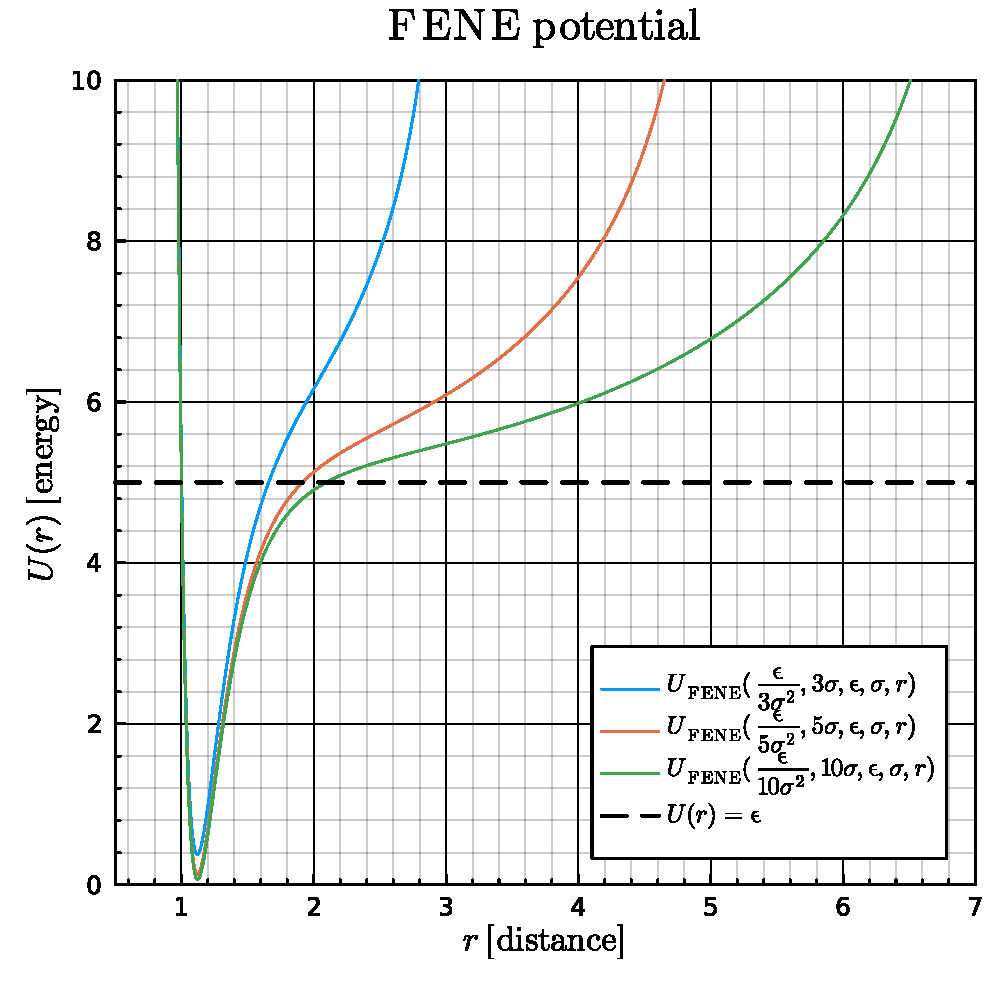
\includegraphics[width=\textwidth]{imgs/hw4/FENEComparison.pdf}
        \caption{~}\label{fig:FENEcomparison}
    \end{subfigure}
    \begin{subfigure}[c]{0.48\textwidth}
        \centering
        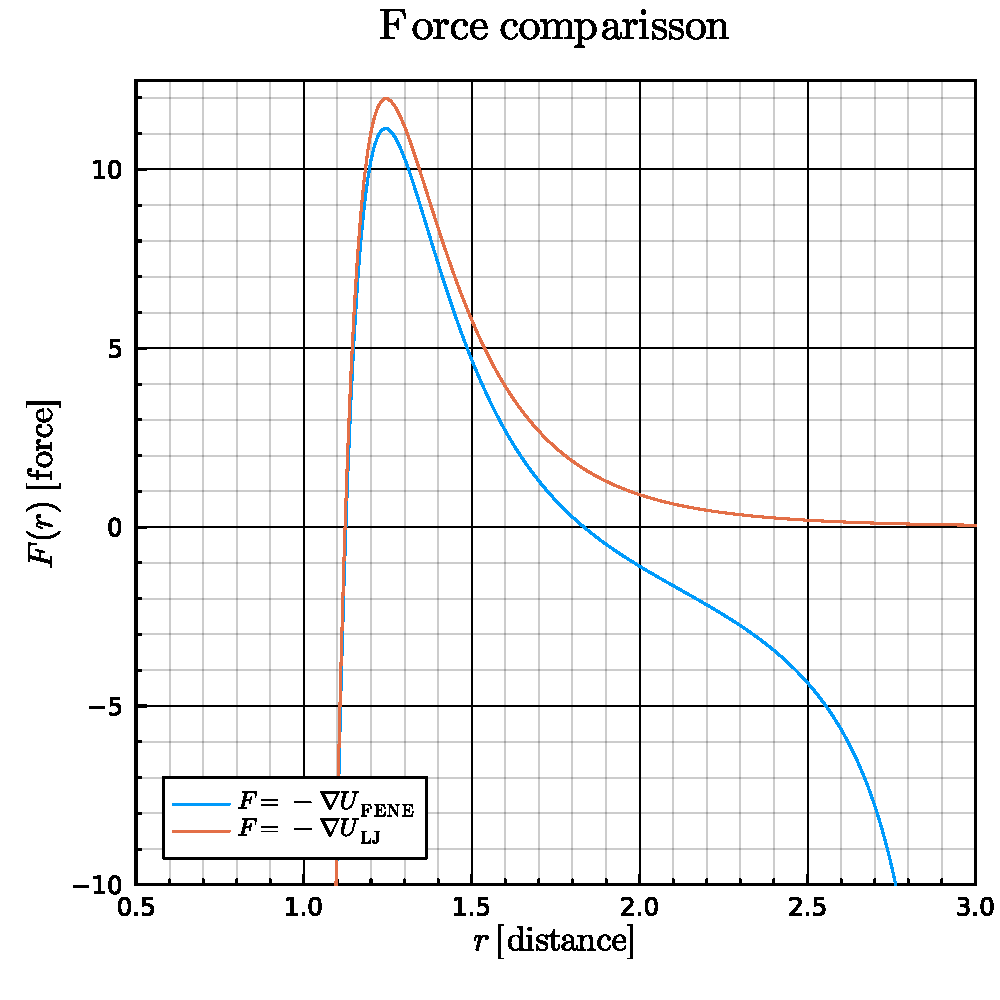
\includegraphics[width=\textwidth]{imgs/hw4/forceComparison.pdf}
        \caption{~}\label{fig:Forcecomparison}
    \end{subfigure}
    %\includegraphics{}
    \caption{
        \ref{fig:FENEcomparison} Comparison of the FENE potential with different $R_{o}$ and $K$ in terms of $\epsilon$ and $\sigma$.
        \ref{fig:Forcecomparison} Comparison of the force due to a FENE potential with a force due to a Lennard-Jones potential with $R_{o} = 3\sigma$ and $K = \epsilon/(3\sigma)^2$.
    }
    \label{fig:ComparisonFENNE-LJ}
\end{figure}

\section{Angular potentials}

Knowing that the FENE potential is going to cause a strong attractive force at a certain distance it is needed to add a restriction in order to prevent the particle chain collapse in a small cluster.
For that potentials with angular dependence are introduce in the script.

As mention in class, the potential with angular dependence used in the simulation are harmonic angle \cite{angle_style_Harmonic_LAMMPSdoc} and dihedral harmonic \cite{dihedral_style_Harmonic_LAMMPSdoc}.
The angle harmonic potential is described with the following equation,
\begin{gather}
    E\qty(\theta) = K\qty(\theta-\theta_{o})^{2}\label{eqn4:anglePotential},
\end{gather}
where $K$ is the energy with units of energy over radian squared and $\theta_{o}$ is the angle of equilibrium.
On the other hand, the dihedral harmonic potential is modeled as,
\begin{gather}
    E\qty(\phi) = K\qty[1+d\cos\qty(n\phi)]\label{eqn4:dihedralPotential},\quad d\in\{1,-1\},~n\in\mathbb{Z}
\end{gather}
where $K$ is the energy. 
The parameter $d$ change the maximum of the function to a minimum when $\phi = \pi$ and the parameter $n$ change the frequency.

Is important to acknowledge that the angle $\theta$ refers to the polar angle and $\phi$ to the azimuth angle in spherical coordinates, hence, introducing both angular potentials will help to introduce restrictions in the behavior of the particle chain.

In figure \ref{fig:angularPotentials} is a comparison of both angular potentials in the angular domain of $0$ to $2\pi$, taking advantage of the periodic pattern of the $\cos$ function.
The angle of equilibrium for the angle harmonic potential is set to $\pi$ and $n$ is set to $1$ for the dihedral harmonic potential for visualization purposes.

\begin{figure}[ht!]
    \centering
    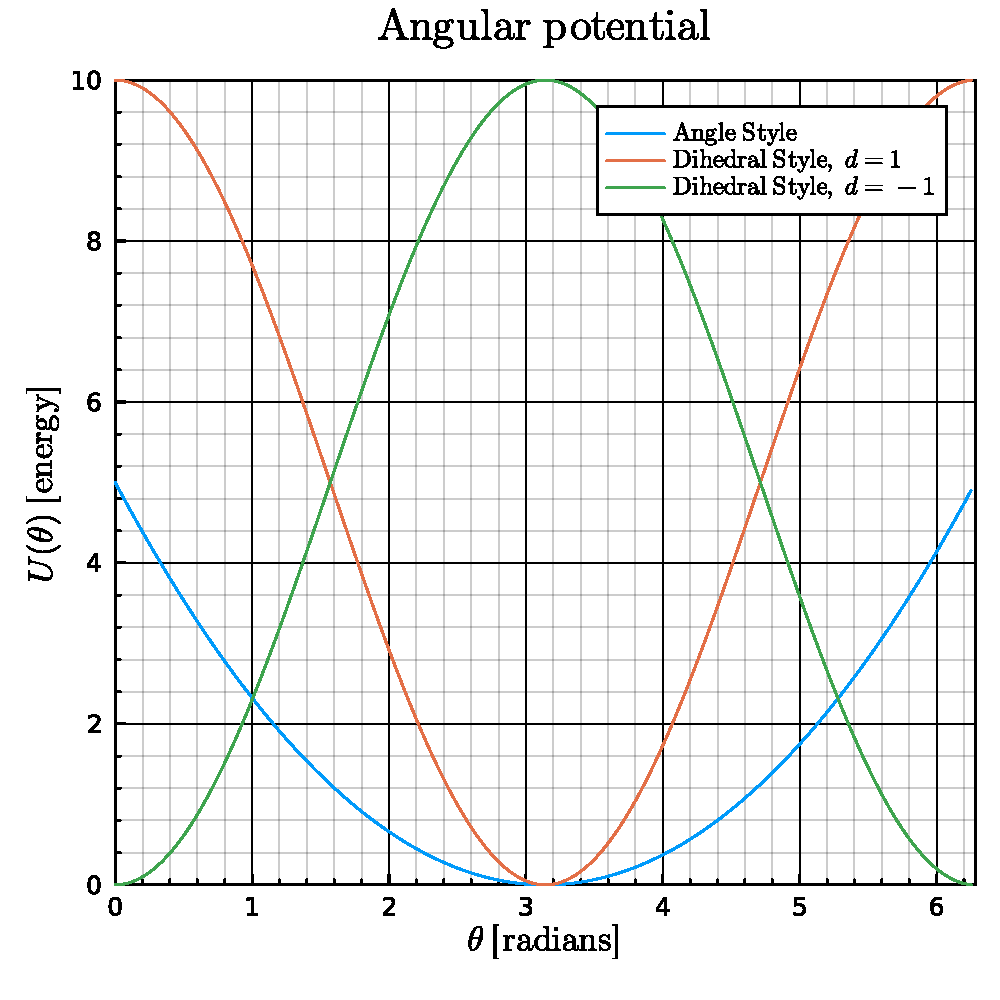
\includegraphics[width=0.5\textwidth]{imgs/hw4/angularPotential.pdf}
    \caption{
        Comparison between angular and dihedral style potentials, with $\theta_{o} = \pi$ and $n = 1$.
        }
    \label{fig:angularPotentials}
\end{figure}

\section{Results}

The main result of the simulation are the trajectories of the polymer chains, hence, in the following link you can access to the animations of the polymer chains:
\href{https://tecmx-my.sharepoint.com/:f:/g/personal/a00827546_tec_mx/Em7ZRtUwkWFJq2eKKiTQE4gBxVktk2Dbfr_g3iGSJvc9cw?email=leogabac%40tec.mx&e=myOo80}{\color{blue}{Access to the animation}}.
On the other hand, in figure \ref{fig:energyAngle} it is shown a comparison of kinetic, potential and total energy of the simulations with polymer chains modeled with angle restriction and angle with dihedral restriction.

As a global characteristic of both systems the tendency of the energies are the same, however the polymers chains modeled with just the angle restriction has more energy than the chains modeled with angle and dihedral restrictions.
This difference makes sense because the second polymer chain has less degrees of fredoom than the first one.

\begin{figure}[ht!]
    \centering
    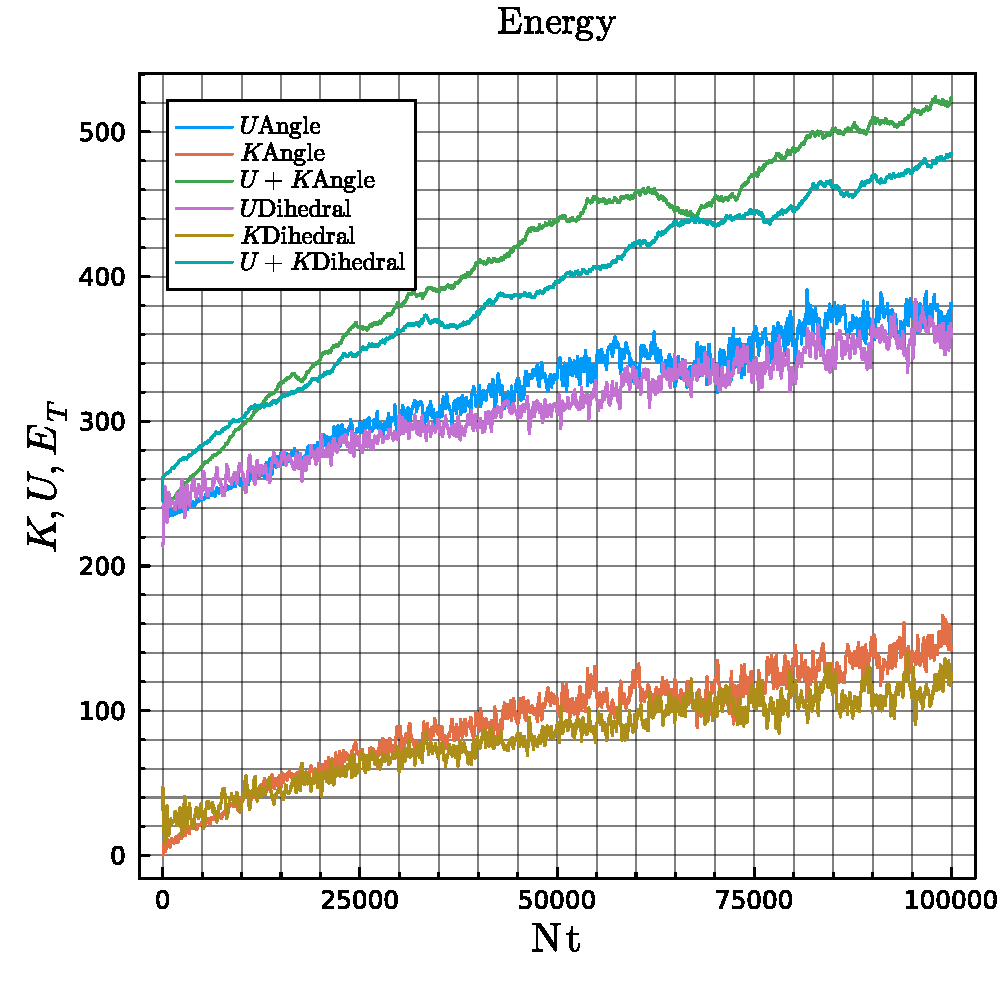
\includegraphics[width=0.8\textwidth]{imgs/hw4/energyComparison.pdf}
    \caption{
        Comparison of kinetic, potential and total energy for simulations of a polymer chain modeled with angle restriction ($U_{\mathrm{Angle}},~K_{\mathrm{Angle}}$) and a polymer chain with angle and dihedral restriction ($U_{\mathrm{Dihedral}},~K_{\mathrm{Dihedral}}$).
    }
    \label{fig:energyAngle}
\end{figure}

%\begin{figure}[ht!]
%    \centering
%    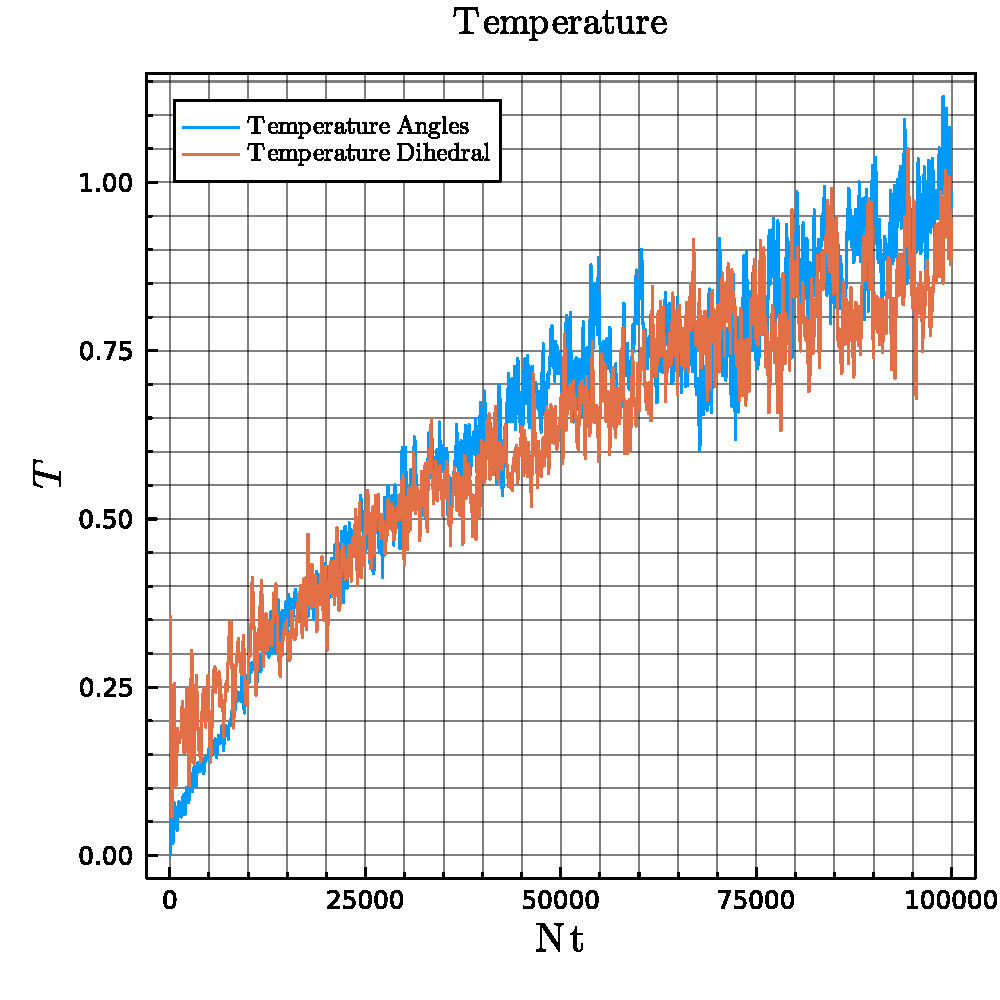
\includegraphics[width=0.8\textwidth]{imgs/hw4/temperatureComparison.pdf}
%    \caption{Temperature with angle restriction}
%    \label{fig:tempAngle}
%\end{figure}


\end{document}